\chapter{Interrupts}
\section{Interrupt Controller}
\label{sec:irq_ctrl}
The interrupt controller features a configurable number of interrupt lines with a configurable amount of priorities.
The configuration follows that of the \procname (see Section \ref{sec:config}).
These intterupts lines need to be asserted for one clock cycle to trigger an interrupt request to the processor core.
Additionally, trap requests from the core are handled (as described in \ref{sec:trap}).

\section{Priority, NMI}
\label{sec:nmi}
The processor features multiple levels of runtime priority (configurable, see Section \ref{sec:config_priowidth}) where a greater number means higher priority.
Additionally, non maskable interrupts (NMI) are supported which are always executed regardless the current processor runtime priority.

The processor starts with the highest possible runtime priority by default to disable interrupts at startup (with the exception of NMI).

This is needed as the stack pointer needs to be set to a valid address before any interrupt (including NMI) can be executed.

\section{Interface and Timing Diagram}
Both ports \inlinevhdl{in\_irq} and \inlinevhdl{out\_irq} (for type definitions see Listing \ref{lst:typedef_irq}) should be connected to a fitting interrupt controller (for example the implementation described in Section \ref{sec:irq_ctrl}).

\begin{vhdl}[Type definitions for Interrupt Controller Ports]{lst:typedef_irq}
-- collection of all signals from the
-- interrupt controller to the core
type irq_core is record
	-- interrupt number of requested interrupt
	num      : unsigned(irq_num_width - 1 downto 0);
	-- priority of requested interrupt
	-- (higher number means higher priority)
	priority : unsigned(irq_prio_width - 1 downto 0);
	-- request signal, active high
	req      : std_logic;
	-- non maskable interrupt flag, active high
	nmi      : std_logic;
end record;

-- collection of all signals from the core
-- to the interrupt controller
type core_irq is record
	-- interrupt acknowledge
	-- high if requested interrupt is processed
	ack      : std_logic;
	-- number of interrupt requested by
	-- internal trap instruction
	trap_num : unsigned(irq_num_width - 1 downto 0);
	-- request signal for internal trap, active high
	trap_req : std_logic;
end record;
\end{vhdl}

\subsection{Interrupt Request}
The external world (i.e. the interrupt controller) can request an interrupt by writing the interrupt number, its priority to \inlinevhdl{in\_irq} and setting the \inlinevhdl{nmi} bit accordingly.
After these are set, \inlinevhdl{req} can be asserted and must be held high until the core acknowledges the interrupt request by asserting \inlinevhdl{ack} for one clock cycle (see Figure \ref{fig:signal_irq_req}).

\begin{figure}[htb]
	\center
	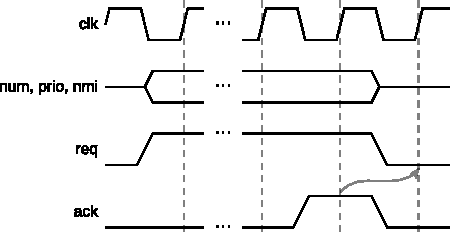
\includegraphics[scale=1]{./figures/signal_irq_req.pdf}
	\caption{Signal Pattern for Interrupt Requests}
	\label{fig:signal_irq_req}
\end{figure}

\subsection{Trap Implementation}
\label{sec:trap}
When executing a trap instruction, an interrupt line to the interrupt controller is asserted for one clock cycle with the interrupt number asserted as well, see Figure \ref{fig:signal_irq_trap}.
Note, that an arbitrary time (and number of instructions) may take place between a trap and the interrupt handler execution.
\begin{figure}[htb]
	\centering
	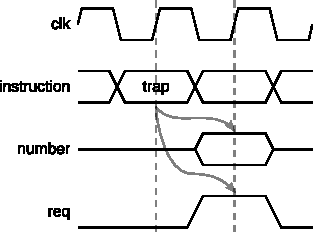
\includegraphics[scale=1]{./figures/signal_irq_trap.pdf}
	\caption{Signal Pattern for Trap Instruction}
	\label{fig:signal_irq_trap}
\end{figure}

\subsection{Processor Interrupt Behavior}
\label{sec:InterruptEntryCPU}
When an interrupt is accepted by the processor, it saves the current PC and status register on the stack.
Then it replaces the runtime priority in the status register with interrupt's priority and replaces the PC with the interupt vector number.

The \textit{reti} instruction reverses this and resturn to the previous executed program.
Note that the processor by itself does not save any registers apart from status register and program counter.
Any other register that needs to be preserved needs to be saved manually.
